\paragraph{SARS and genetic algorithms. [FRANK]}
\citeauthor{Yan2008} report in \cite{Yan2008} a epidemic model for
Severe acute respiratory syndrome (SARS). They use quarantine and isolation as
mitigation controls. The authors propose sub-optimal control policies and
perform numeric simulations with genetic algorithms. The
controlled version used in the mentioned reference reads:
%
%
\begin{equation}
	\begin{aligned}
		\dfrac{dS}{dt} &=
			\Lambda 
			-\dfrac{
				S
				\left(
					\beta I 
					+ \mathcal{E}_E  \beta E
					+ \mathcal{E}_Q  \beta Q
					+ \mathcal{E}_J  \beta J
				\right)
			}{N}
			- \mu S,
		\\
		\dfrac{dE}{dt} &=
			p +
			\dfrac{
				\beta S
				\left(
					\beta I 
						+ \mathcal{E}_E \beta E
						+ \mathcal{E}_Q \beta Q
						+ \mathcal{E}_J \beta J
				\right)
			}{N}
			-(
				u_1(t) + k_1 + \mu
			)E,
		\\
		\dfrac{dQ}{dt} &=
			u_1(t) E 
			- (k_2 + \mu) Q
		\\
		\dfrac{dI}{dt} &=
			k_1 E 
			-(u_2(t) + d_1  + \sigma_1 + \mu) I,
		\\
		\dfrac{dJ}{dt} &=
			u_2(t) I 
			+ k_2 Q
			- (d_2 + \sigma_2 + \mu) J,
		\\
		\dfrac{dR}{dt} &=
			\sigma_1 I
			+\sigma_2 J
			- \mu R.
	\end{aligned}
\end{equation}
The control variable $u_1$ denotes the proportion of quarantining people 
who had contact with an infected person inside of a quarantining program or
educational campaigns. Control $u_2$ models the proportion of symptomatic 
population which are in a isolation program.
\begin{table}
	\begin{center}
		\begin{tabular}{@{}rll@{}} 
			$S$: & Susceptible individuals 
			\\
			$E$: & Asymptomatic individuals who have been 
			\\
			   & exposed to the virus but have not yet developed 
			\\
			   & clinical symptoms of SARS 
			\\
			$Q$: & Quarantine individuals
			\\
			$I$: & Symptomatic 
			\\
			$J$: & Isolated
			\\
			$R$: & Recovered
			\\
				& $N = S + E + Q + I + J + R$.
		\end{tabular}
	\end{center}
\end{table}
\begin{figure}
  \centering
  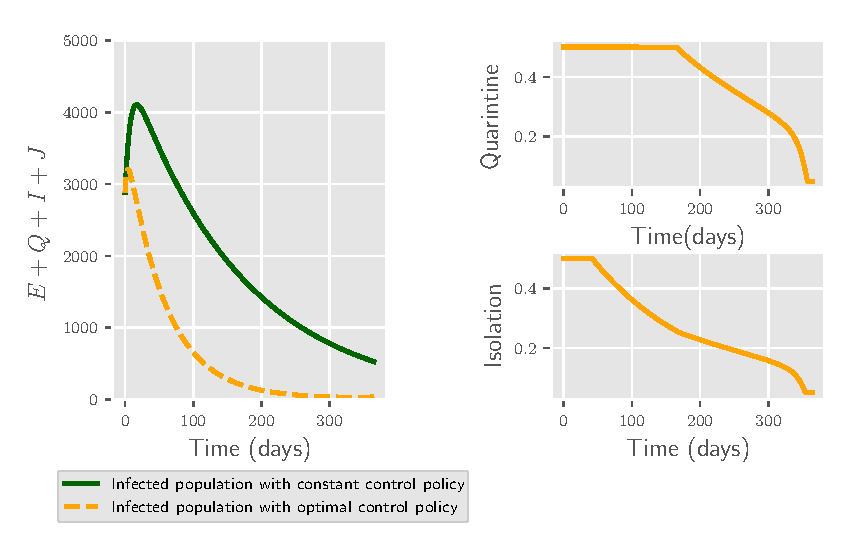
\includegraphics[width=0.7\linewidth]{Figures/figure_1_sars}
  \caption{}
  \label{fig:figure1sars}
\end{figure}


\begin{figure}
  \centering
  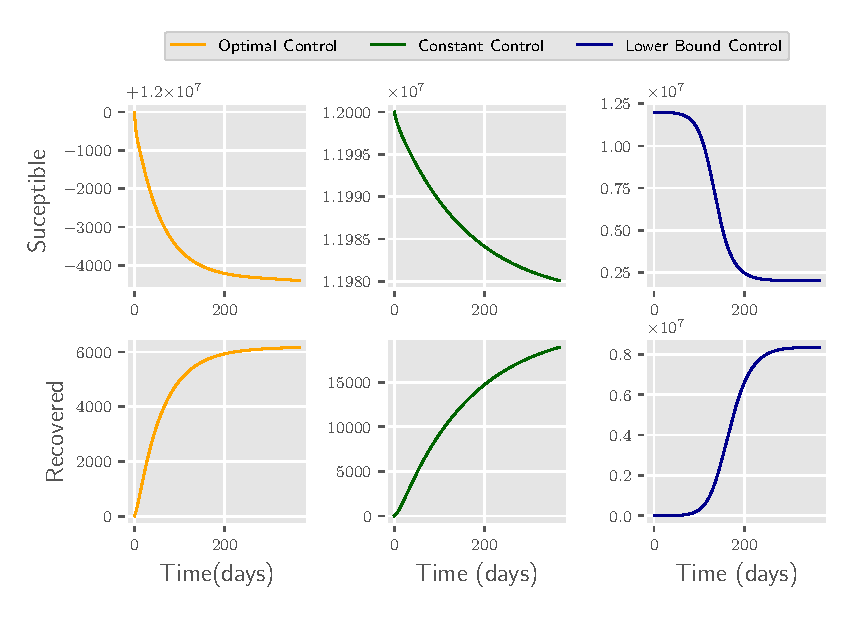
\includegraphics[width=0.7\linewidth]{Figures/figure_2_sars}
  \caption{}
  \label{fig:figure2sars}
\end{figure}

\begin{figure}
  \centering
  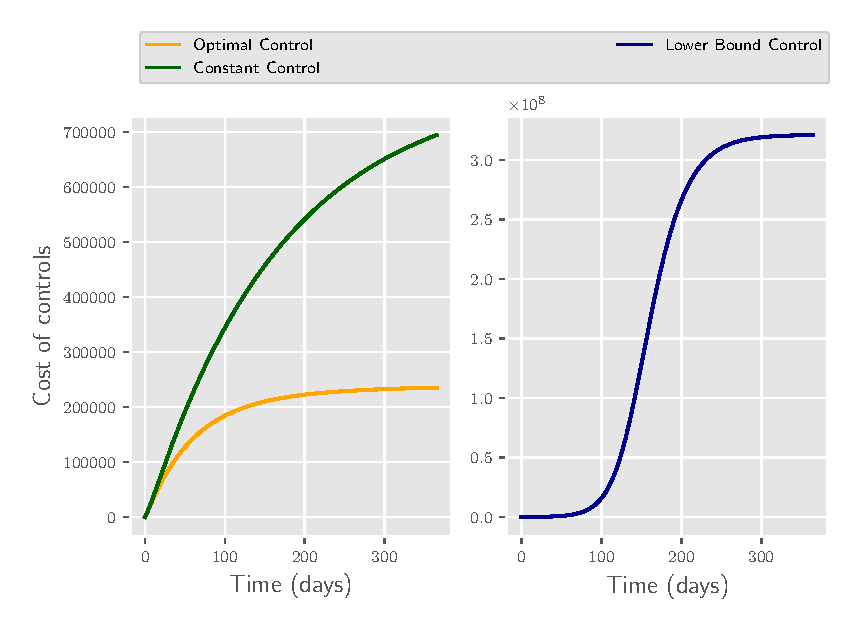
\includegraphics[width=0.7\linewidth]{Figures/figure_3_sars}
  \caption{}
  \label{fig:figure3sars}
\end{figure}